\begingroup
\graphicspath{{../prob_6/Figures/}}


\subsection{Step 1: GAN Training and Initial Generation}

A Generative Adversarial Network (GAN) was trained using a reduced dataset of 350 real samples per digit. The goal was to generate synthetic handwritten digits resembling the MNIST dataset.

As seen in Figure~\ref{fig:gan_samples}, the GAN consisted of a convolutional discriminator and a transposed convolutional generator. The training process was conducted for several epochs until visually acceptable digit-like samples were obtained.

The generated images were slightly blurred but still recognizable, indicating that the GAN successfully captured the general structure of handwritten digits.

\begin{figure}[H]
    \centering
    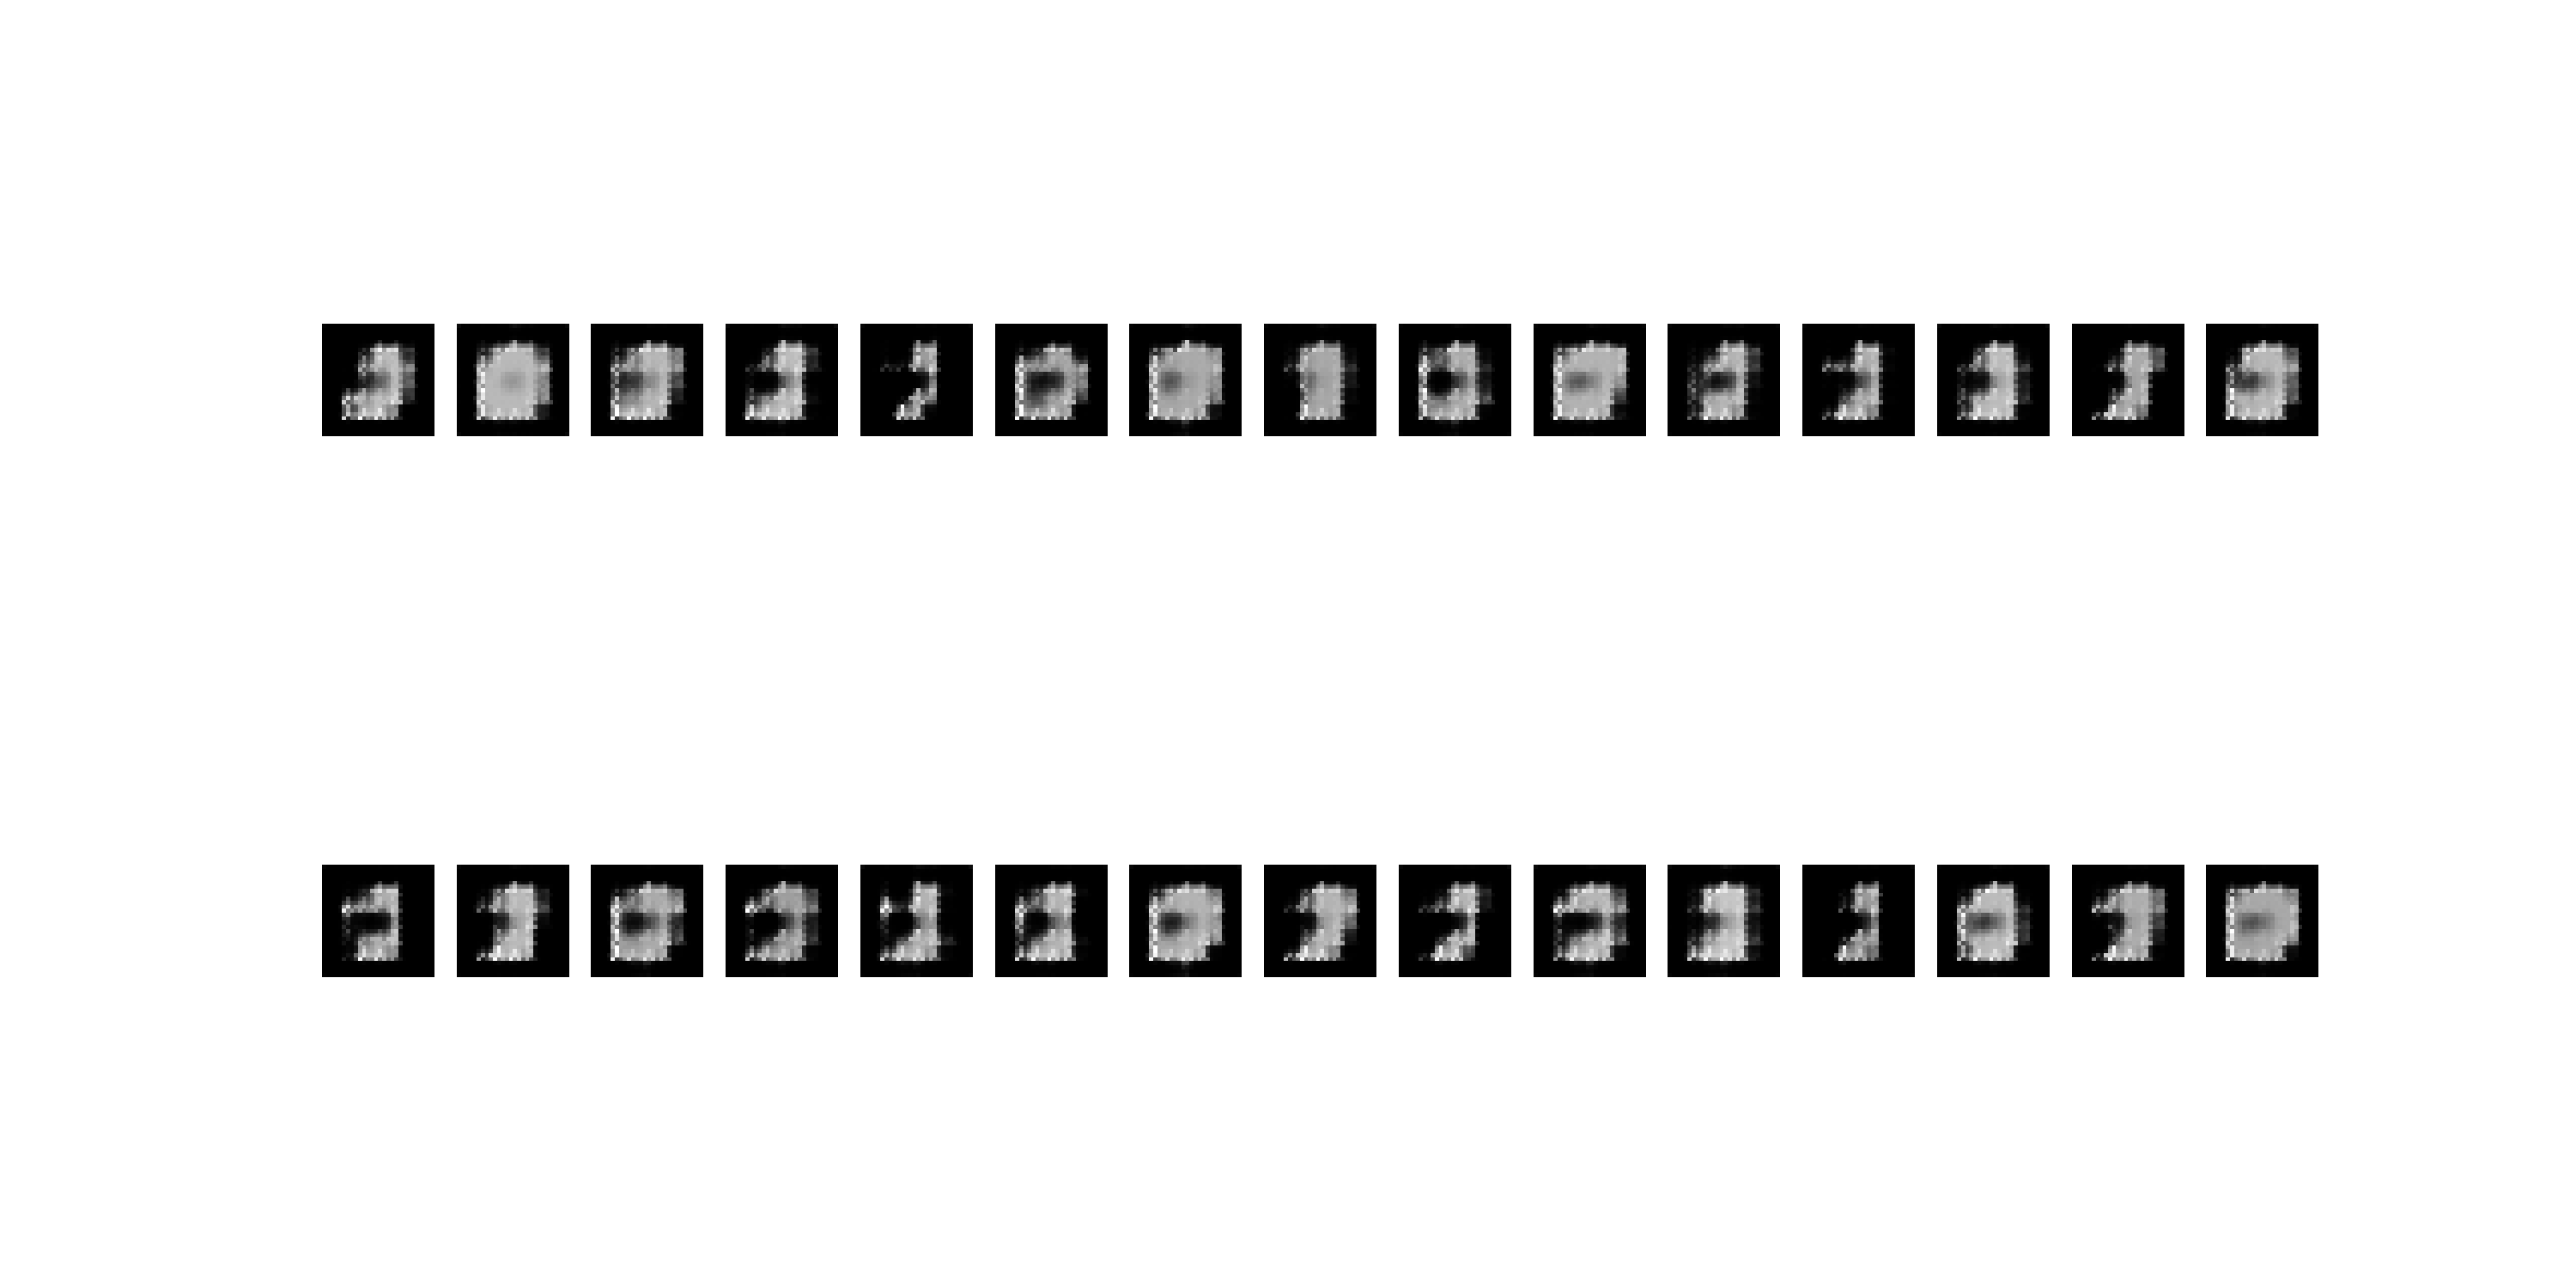
\includegraphics[width=0.6\linewidth]{gan_generated_samples.png}
    \caption{Samples generated by the GAN}
    \label{fig:gan_samples}
\end{figure}

\subsection{Step 2: Effect of Synthetic Data on Classification Accuracy}

The generated data was combined with different amounts of real data (350, 750, and 1000 samples per digit). The classification accuracy for each configuration is summarized in Table~\ref{tab:gan_results} and visualized in Figure~\ref{fig:gan_results}.

\begin{table}[H]
\centering
\caption{Accuracy for different combinations of real and GAN-generated data}
\label{tab:gan_results}
\begin{tabular}{|c|c|c|}
\hline
\textbf{Real per digit} & \textbf{GAN per digit} & \textbf{Accuracy} \\ \hline
350 & 0    & 0.9548 \\ \hline
350 & 1000 & 0.9676 \\ \hline
350 & 1500 & 0.9651 \\ \hline
350 & 2000 & 0.9573 \\ \hline
750 & 0    & 0.9733 \\ \hline
750 & 1000 & 0.9719 \\ \hline
750 & 1500 & 0.9752 \\ \hline
750 & 2000 & 0.9638 \\ \hline
1000 & 0    & 0.9690 \\ \hline
1000 & 1000 & 0.9775 \\ \hline
1000 & 1500 & 0.9735 \\ \hline
1000 & 2000 & 0.9740 \\ \hline
\end{tabular}
\end{table}

\begin{figure}[H]
    \centering
    
\includegraphics[width=0.85\linewidth]{results_plot.png}
    \caption{Accuracy vs. GAN-generated samples per digit for different real dataset sizes}
    \label{fig:gan_results}
\end{figure}

From Table~\ref{tab:gan_results} and Figure~\ref{fig:gan_results}, the following observations can be made:

\begin{itemize}
    \item Adding synthetic data significantly improves performance when the real dataset is small (350 samples).
    \item The best improvement is achieved around 1000 generated samples per digit.
    \item Increasing synthetic data beyond this point does not improve accuracy and may slightly degrade performance.
    \item This behavior is due to the limited quality and diversity of GAN-generated samples.
\end{itemize}

\subsection{Step 3: Reducing the Need for Real Data}

The baseline case using only real data (1000 samples per digit) achieved an accuracy of approximately $96.9\%$.

When using only 350 real samples combined with 1000 GAN-generated samples, the accuracy increased to $96.76\%$, which is very close to the full real-data scenario.

This demonstrates that GAN-generated data can effectively compensate for limited real data.

However, excessive use of synthetic data leads to diminishing returns due to artifacts and reduced diversity in generated images.

\subsection{Discussion}

The results confirm that GANs can reduce the dependency on real data while maintaining high accuracy.

\begin{itemize}
    \item Synthetic data is most beneficial when real data is limited.
    \item There exists an optimal balance between real and generated data.
    \item Over-reliance on synthetic data can negatively impact performance.
\end{itemize}

\endgroup